%!TEX root = ./main.tex

Al ser preliminares no se entrara tanto en detalle en algunos resultados, mas se presentaran cálculos básicos necesarios para posteriormente poder calcular directamente en los complementos de los Nudos, por lo que al trabajar con las proyecciones de nudos en $S^2$ (Plano) es natural empezar entendiendo nociones básicas de la geometría hiperbólica en dimensión 2.

\begin{definition}
    El espacio hiperbólico 2-dimensional $\mathbb{H}^2$ es el conjunto de puntos
    $$\mathbb{H}^2:=\{z\in\C:\Im(z)>0\},$$
    Donde si $z=x+iy$, dotamos al espacio de una métrica dada por
    $$ds^2=\frac{dx^2+dy^2}{y^2}$$
\end{definition}
Esta métrica se puede interpretar como la métrica usual de el plano $dx^2+dy^2$ re escalada por el factor. Note en particular que al ser puntos del plano complejo tenemos dos interpretaciones, como un punto $z\in\C$ o como $(x,y)\in\R^2$, ambas serán útiles dependiendo del contexto por lo que cambiaremos entre ellas según convenga.\\

Esta idea de métrica y del espacio hiperbólico se pueden ver mas a fondo desde la perspectiva de la geometría Riemanniana, mas debido a que esto es un curso completo nos quedaremos con las formulas fundamentales, primero la que nos permite calcular longitudes.
\begin{definition}
    Sea $\gamma:[a.b]\to \mathbb{H}^2$ una curva diferenciable, definimos la longitud de la curva como 
    $$|\gamma|=\int_a^b\frac{1}{\gamma_y(s)}\sqrt{(\gamma^{\prime}_x(s))^2+(\gamma^{\prime}_y(s))^2}\,ds$$
    donde $\gamma(s)=(\gamma_x(s),\gamma_y(s)).$
\end{definition}


\begin{eg}
    Las longitudes mas básicas de calcular en la geometría euclidiana usual son las rectas horizontales y verticales, así que hagamos lo mismo. Considere el segmento que va del punto $(0,h)$ a el punto $(1,h)$, este segmento esta parametrizado por $\gamma(t)=(t,h)$ con $t\in[0,1]$, así obtenemos
    $$|\gamma|=\int_0^1\frac{1}{h}\sqrt{1^2+0^2}\,ds=\frac{1}{h}$$
    Que es lo esperado la distancia usual del segmento euclidiano (1) re escalada por la altura. Observe que esto nos dice que cuando $h\to\infty$ los puntos a pesar de que en el semiplano superior se ven a una distancia fija en realidad se están acercando, de manera similar si $h\to 0^+$ los puntos se alejan.\\

    Ahora consideremos una recta vertical, es decir una recta parametrizada por $\gamma(t)=(x,t)$, donde $x$ esta fijo y $t\in[a,b]$, por la formula tenemos
    $$|\gamma|=\int_a^b\frac{1}{s}\sqrt{0^2+1^2}\,ds=\log\left(\frac{b}{a}\right).$$
    De aquí podemos observar que si fijamos $a$ y $b\to\infty$ tenemos que estos se alejan, y si $b$ es fijo y $a\to 0^+$ la distancia también tiende a infinito.
    \end{eg}

    Este comportamiento que se sale de la intuición del dibujo euclideo también se traslada a la siguiente formula para calcular áreas y el calculo particular.

    \begin{definition}
        Dada una región $R\subset \bb{H}^2$, definimos el área como
        $$\text{area}(R)=\int_R\frac{1}{y^2}dR.$$
    \end{definition}
    \begin{eg}
        Como ejemplo de calculo considere la siguiente región
         $$R=\{(x,y)\in \bb{R}^2: 0\leq x\leq 1,y\geq 1\},$$
         Esto es una franja que se extiende al infinito, usando la formula
         $$\text{area}(R)=\int_0^1\int_1^\infty\frac{1}{y^2}\,dydx=\int_0^11\,dx=1.$$
         Esto nos muestra como regiones euclideas con área infinita pueden tener área finita, esto sera excesivamente relevante cuando hablemos del volumen hiperbólico de un nudo.
    \end{eg}

    Observe que a pesar de no pertenecer al espacio hiperbólico, la recta real y acercarse al infinito nos da información geométrica del mismo, por esto es común otorgarles nombre propio para referirse a ambos en conjunto.

    \begin{definition}
        Llamamos a $\bb{R}\cup\{\infty\}$ la frontera en el infinito de $\bb{H}^2$, y la denotamos por $\partial_\infty\bb{H}^2$
    \end{definition}

    Una observación particular es que al igual que antes por proyección estereográfica tenemos que $\partial_\infty\bb{H}^2\cong S^1$.\\

    Entre estos puntos de la frontera y todos los puntos que se encuentran en $\bb{H}^2$ nos gustaría encontrar aquellas curvas que minimizan la distancia entre puntos, en el caso euclideo estas siempre son rectas, pero en general no tendrían por que serlo en otras métricas, así definimos la siguiente nocion
    \begin{definition}
        Dados puntos  $p,q\in\bb{H}^2$ decimos que una geodésica entre estos puntos es una curva $\gamma$ que justamente minimiza $|\gamma|$. Una geodésica infinita es una curva $\gamma:\bb{R}\to \bb{H}^2$ tal que dado un intervalo $[s,t]$, la curva $\gamma([s,t])$ es una geodésica entre $\gamma(s)$ y $\gamma(t).$
    \end{definition}

    Al igual que en el caso euclideo las geodésicas tienen una forma particular en el caso hiperbólico, mas son diferentes

    \begin{theorem}
        Las geodésicas infinitas en $\bb{H}^2$ consiste de lineas verticales cuando dos puntos comparten parte real y de semicírculos con centro en la recta real para el otro caso.
    \end{theorem}

    Algo particular a notar es que estas geodésicas se intersectan con $\partial_\infty\bb{H}^2$ en ángulos rectos.\\

    \begin{definition}
        Una isometria $\phi:\bb{H}^2\to\bb{H}^2$ es un difeomorfismo tal que preserva la métrica de $\bb{H}^2$
    \end{definition}

    Claramente estas dos ultimas definiciones se pueden dar en contextos mas generales pero nos quedaremos en nuestro caso hiperbólico, dicho esto en particular nos interesan la isometrias que preservan la orientación, si juntamos todas estas isometrias estas forman un grupo con una descripción particular.
    \begin{theorem}
        El grupo de isometrias de $\bb{H}^2$ es generado por reflexiones a través geodésicas, en particular si miramos aquellas que preservan la orientación es el grupo dado por las siguientes transformaciones
        $$z\mapsto\frac{az+b}{cz+d},$$
        donde $a,b,c,d\in\bb{R}$ y $ad-bc>0.$
    \end{theorem}
    Estas transformaciones se conocen como transformaciones lineales fraccionarias. Note en particular si cada coeficiente lo normalizamos por $\sqrt{ad-bc}$ (que no afecta la transformación) podemos entender estas transformaciones como la acción del grupo $PSL(2,\bb{R})$ sobre $\bb{H}^2$ donde la acción esta dada por
    $$\begin{pmatrix}
        a&b\\
        c&d
    \end{pmatrix}\cdot z=\frac{az+b}{cz+d}.$$
    Este tipo de transformaciones son particularmente útiles ya que permiten escoger a donde llevamos un punto particular, esto se ve en el siguiente lema que es bastante útil.
    \begin{lemma}
        Dados tres puntos diferentes $z_1,z_2z_3\in\partial_\infty\bb{H}^2$, existe una isometria que preserva la orientación tal que tal que 
        $$z_i\mapsto\begin{cases}
            1, & i=1\\
            0, & i=2\\
            \infty & i=3
        \end{cases}$$
    \end{lemma}
    \begin{proof}
       El detalle mas importante que hay que cuidar es el tema de la orientación (mantener el signo del determinante positivo), si ningún punto es $\infty$ observe que son tres puntos en la recta real, así considere
       $$z\mapsto \frac{z_1-z_3}{z_1-z_2}\frac{z-z_2}{z-z_3}$$ 
       Note que 
       $$z_1\mapsto \frac{z_1-z_3}{z_1-z_2}\frac{z_1-z_2}{z_1-z_3}=1,\quad z_2\mapsto \frac{z_1-z_3}{z_1-z_2}\frac{z_2-z_2}{z_2-z_3}=0,\quad z_3\mapsto \frac{z_1-z_3}{z_1-z_2}\frac{z_3-z_2}{z_3-z_3}=\infty.$$
       Ahora note que el producto de coeficientes es $$(z_1-z_3)(-z_3)(z_1-z_2)-(-z_2)(z_1-z_3)(z_1-z_2)=(z_1-z_3)(z_1-z_2)(z_2-z_3).$$
       Observe que el signo depende completamente de el orden en el que uno etiquete los puntos, en particular si uno los etiqueta en un sentido antihorario partiendo desde $z_1$ claramente es positivo.\\

       En el caso que $z_i=\infty$ para alguno de los $i$, la isometria es la siguiente para cada caso
       $$z\mapsto\begin{cases}
           \dfrac{z-z_2}{z-z_3},&i=1\\
           \\
           \dfrac{z_1-z_3}{z-z_3},&i=2\\
           \\
           \dfrac{z-z_2}{z_1-z_2},&i=3
       \end{cases}$$
       Este ultimo es fácil verificar nuevamente que enviá los puntos a lo enunciado y el determinante resulta siempre positivo por la manera en que organizamos los puntos.

    \end{proof}
    Estas isometrias dan mucha facilidad no solo para cálculos sino también para algunos hechos de la geometría del espacio.
    \begin{corollary}
        Siempre existe una isometria tal que dados tres puntos diferentes $z_1,z_2,z_3$ en la frontera al infinito pueden ser enviados a otros tres diferentes $z_1^\prime,z_2^\prime,z_3^\prime$ también en la frontera al infinito.
    \end{corollary}
    \begin{corollary}
        Dadas dos geodésicas $l_1,l_2$ en $\bb{H}^2$ solo hay tres posibilidades
        \begin{itemize}
            \item $l_1\cap l_2=\{x\}\subset \bb{H}^2.$
            \item $l_1\cap l_2=\{x\}\subset \partial_\infty\bb{H}^2.$
            \item $ l_1\cap l_2=\varnothing.$ 
        \end{itemize}
    \end{corollary}
    \begin{eg}
       Previamente habíamos hallado la distancia entre dos puntos con la misma parte real (esto ya que la recta vertical si es una geodésica), pero por ejemplo para por ejemplo el punto $(0,h)$ y $(1,h)$ la longitud de ese segmento es claro que no es la mas corta, la mas corta es la que esta dada por el segmento del semicírculo que contiene a estos dos puntos, este circulo es 
       $\left(x-\dfrac{1}{2}\right)^2+y^2=h^2+\dfrac{1}{4}.$
       Este circulo interseca a la frontera en 
       $x=\dfrac{1}{2}\pm\sqrt{h^2+\dfrac{1}{4}},$ 
       esto es haciendo $y=0$, luego hay dos estrategias para calcular la distancia, una seria hallar la integral paramétrica, la otra es usar la isometria hallada previamente para convertir esta geodésica en la recta vertical de $0$ a $\infty$, en el lenguaje de la prueba si tomamos
       $z_1=\infty,\quad z_2=\dfrac{1}{2}+\sqrt{h^2+\dfrac{1}{4}},\quad z_3=\dfrac{1}{2}-\sqrt{h^2+\dfrac{1}{4}},$
       la transformación 
       $z\mapsto \dfrac{z-z_2}{z-z_3},$ hace justamente lo que queremos, Luego la imagen de $ih$ y $1+ih$ es respectivamente
       $a=\dfrac{ih-z_2}{ih-z_3},\quad b=\dfrac{1+ih-z_2}{1+ih-z_3},$
      Así por el calculo hecho previamente sabemos que la distancia entre estos dos puntos es $\pm\log\left(\dfrac{\Im(b)}{\Im(a)}\right)$, el $\pm$ esta ya que depende de que parte imaginaria sea mayor, y como las isometrias preservan distancias tenemos la distancia explicita entre los puntos originales. 
    \end{eg}

    \begin{figure}[H]
    \centering
    
%!TEX root = ./main.tex



\tikzset{every picture/.style={line width=0.75pt}} %set default line width to 0.75pt        

\begin{tikzpicture}[x=0.75pt,y=0.75pt,yscale=-1,xscale=1]
%uncomment if require: \path (0,877); %set diagram left start at 0, and has height of 877

%Shape: Arc [id:dp3323452367299544] 
\draw  [draw opacity=0] (247.5,190) .. controls (247.5,158.24) and (273.24,132.5) .. (305,132.5) .. controls (336.76,132.5) and (362.5,158.24) .. (362.5,190) -- (305,190) -- cycle ; \draw   (247.5,190) .. controls (247.5,158.24) and (273.24,132.5) .. (305,132.5) .. controls (336.76,132.5) and (362.5,158.24) .. (362.5,190) ;  
%Straight Lines [id:da5286576515069806] 
\draw    (133,190) -- (477,190) ;
\draw [shift={(480,190)}, rotate = 180] [fill={rgb, 255:red, 0; green, 0; blue, 0 }  ][line width=0.08]  [draw opacity=0] (8.93,-4.29) -- (0,0) -- (8.93,4.29) -- cycle    ;
\draw [shift={(130,190)}, rotate = 0] [fill={rgb, 255:red, 0; green, 0; blue, 0 }  ][line width=0.08]  [draw opacity=0] (8.93,-4.29) -- (0,0) -- (8.93,4.29) -- cycle    ;
%Straight Lines [id:da6944501524708641] 
\draw    (280,53) -- (280,190) ;
\draw [shift={(280,50)}, rotate = 90] [fill={rgb, 255:red, 0; green, 0; blue, 0 }  ][line width=0.08]  [draw opacity=0] (8.93,-4.29) -- (0,0) -- (8.93,4.29) -- cycle    ;
%Straight Lines [id:da6550119981386697] 
\draw    (130,140) -- (460,140) ;
%Shape: Arc [id:dp7496478031646566] 
\draw  [draw opacity=0][line width=2.25]  (279.69,138.36) .. controls (287.33,134.61) and (295.92,132.5) .. (305,132.5) .. controls (314.52,132.5) and (323.49,134.81) .. (331.4,138.9) -- (305,190) -- cycle ; \draw  [color={rgb, 255:red, 74; green, 144; blue, 226 }  ,draw opacity=1 ][line width=2.25]  (279.69,138.36) .. controls (287.33,134.61) and (295.92,132.5) .. (305,132.5) .. controls (314.52,132.5) and (323.49,134.81) .. (331.4,138.9) ;  

% Text Node
\draw (352,190.4) node [anchor=north west][inner sep=0.75pt]    {$z_{2}$};
% Text Node
\draw (242,190.4) node [anchor=north west][inner sep=0.75pt]    {$z_{3}$};
% Text Node
\draw (261,122.4) node [anchor=north west][inner sep=0.75pt]    {$ih$};
% Text Node
\draw (337,122.4) node [anchor=north west][inner sep=0.75pt]    {$1+ih$};


\end{tikzpicture}
        \caption{Geodésica que contiene a los puntos}
    \end{figure}

    Con estas herramientas se ve un camino mejor hacia los cálculos, pero recordemos hacia donde vamos, la idea es poder calcular de alguna forma sobre las descomposiciones de los complementos en $S^3$ de nudos/enlaces, estos complementos generaran regiones y estructuras particulares en $S^3$ por lo que necesitamos subir de dimensión e intentar ver áreas y volúmenes, las siguientes definiciones empiezan a ir en esa dirección.

    \begin{definition}
        Un triangulo ideal en $\bb{H}^2$ es un triangulo donde sus tres aristas son geodésicas y su vértices se encuentran en $\partial_\infty\bb{H}^2.$
    \end{definition}

        \begin{figure}[H]
        \centering
        
%!TEX root = ./main.tex



\tikzset{every picture/.style={line width=0.75pt}} %set default line width to 0.75pt        

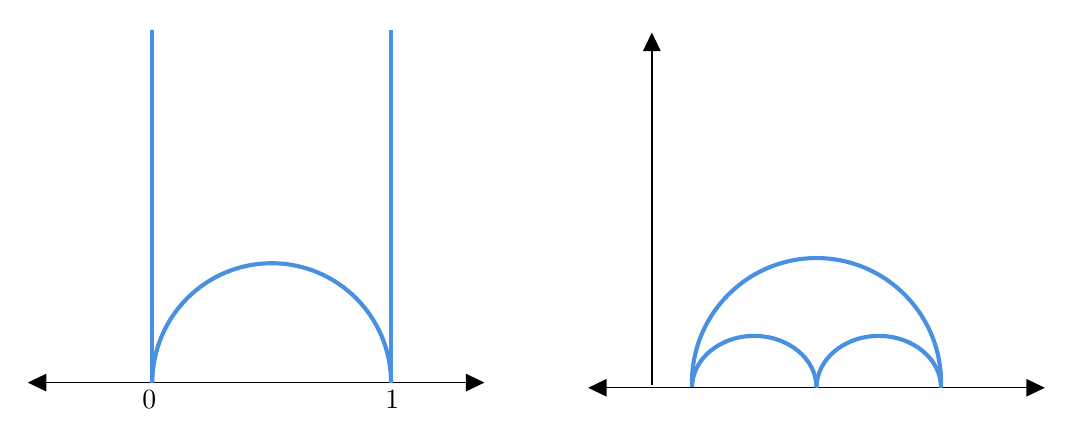
\begin{tikzpicture}[x=0.75pt,y=0.75pt,yscale=-1,xscale=1]
%uncomment if require: \path (0,877); %set diagram left start at 0, and has height of 877

%Shape: Arc [id:dp3323452367299544] 
\draw  [draw opacity=0][line width=1.5]  (140,200) .. controls (140,200) and (140,200) .. (140,200) .. controls (140,168.24) and (165.74,142.5) .. (197.5,142.5) .. controls (229.26,142.5) and (255,168.24) .. (255,200) -- (197.5,200) -- cycle ; \draw  [color={rgb, 255:red, 74; green, 144; blue, 226 }  ,draw opacity=1 ][line width=1.5]  (140,200) .. controls (140,200) and (140,200) .. (140,200) .. controls (140,168.24) and (165.74,142.5) .. (197.5,142.5) .. controls (229.26,142.5) and (255,168.24) .. (255,200) ;  
%Straight Lines [id:da5286576515069806] 
\draw    (83,200) -- (297,200) ;
\draw [shift={(300,200)}, rotate = 180] [fill={rgb, 255:red, 0; green, 0; blue, 0 }  ][line width=0.08]  [draw opacity=0] (8.93,-4.29) -- (0,0) -- (8.93,4.29) -- cycle    ;
\draw [shift={(80,200)}, rotate = 0] [fill={rgb, 255:red, 0; green, 0; blue, 0 }  ][line width=0.08]  [draw opacity=0] (8.93,-4.29) -- (0,0) -- (8.93,4.29) -- cycle    ;
%Straight Lines [id:da6944501524708641] 
\draw [color={rgb, 255:red, 74; green, 144; blue, 226 }  ,draw opacity=1 ][line width=1.5]    (140,30) -- (140,200) ;
%Straight Lines [id:da7691230862880515] 
\draw [color={rgb, 255:red, 74; green, 144; blue, 226 }  ,draw opacity=1 ][line width=1.5]    (255,30) -- (255,200) ;
%Shape: Arc [id:dp4258690964395112] 
\draw  [draw opacity=0][line width=1.5]  (400,202.5) .. controls (400,202.5) and (400,202.5) .. (400,202.5) .. controls (400,188.69) and (413.43,177.5) .. (430,177.5) .. controls (446.57,177.5) and (460,188.69) .. (460,202.5) -- (430,202.5) -- cycle ; \draw  [color={rgb, 255:red, 74; green, 144; blue, 226 }  ,draw opacity=1 ][line width=1.5]  (400,202.5) .. controls (400,202.5) and (400,202.5) .. (400,202.5) .. controls (400,188.69) and (413.43,177.5) .. (430,177.5) .. controls (446.57,177.5) and (460,188.69) .. (460,202.5) ;  
%Straight Lines [id:da8977320996545466] 
\draw    (353,202.5) -- (567,202.5) ;
\draw [shift={(570,202.5)}, rotate = 180] [fill={rgb, 255:red, 0; green, 0; blue, 0 }  ][line width=0.08]  [draw opacity=0] (8.93,-4.29) -- (0,0) -- (8.93,4.29) -- cycle    ;
\draw [shift={(350,202.5)}, rotate = 0] [fill={rgb, 255:red, 0; green, 0; blue, 0 }  ][line width=0.08]  [draw opacity=0] (8.93,-4.29) -- (0,0) -- (8.93,4.29) -- cycle    ;
%Shape: Arc [id:dp38871258976776124] 
\draw  [draw opacity=0][line width=1.5]  (460,202.5) .. controls (460,202.5) and (460,202.5) .. (460,202.5) .. controls (460,188.69) and (473.43,177.5) .. (490,177.5) .. controls (506.57,177.5) and (520,188.69) .. (520,202.5) -- (490,202.5) -- cycle ; \draw  [color={rgb, 255:red, 74; green, 144; blue, 226 }  ,draw opacity=1 ][line width=1.5]  (460,202.5) .. controls (460,202.5) and (460,202.5) .. (460,202.5) .. controls (460,188.69) and (473.43,177.5) .. (490,177.5) .. controls (506.57,177.5) and (520,188.69) .. (520,202.5) ;  
%Shape: Arc [id:dp5339401693658827] 
\draw  [draw opacity=0][line width=1.5]  (400,200) .. controls (400,166.86) and (426.86,140) .. (460,140) .. controls (493.14,140) and (520,166.86) .. (520,200) -- (460,200) -- cycle ; \draw  [color={rgb, 255:red, 74; green, 144; blue, 226 }  ,draw opacity=1 ][line width=1.5]  (400,200) .. controls (400,166.86) and (426.86,140) .. (460,140) .. controls (493.14,140) and (520,166.86) .. (520,200) ;  
%Straight Lines [id:da11869494313797047] 
\draw [color={rgb, 255:red, 0; green, 0; blue, 0 }  ,draw opacity=1 ][line width=0.75]    (380.67,34.33) -- (380.67,201.33) ;
\draw [shift={(380.67,31.33)}, rotate = 90] [fill={rgb, 255:red, 0; green, 0; blue, 0 }  ,fill opacity=1 ][line width=0.08]  [draw opacity=0] (8.93,-4.29) -- (0,0) -- (8.93,4.29) -- cycle    ;

% Text Node
\draw (134,202.4) node [anchor=north west][inner sep=0.75pt]    {$0$};
% Text Node
\draw (251,202.4) node [anchor=north west][inner sep=0.75pt]    {$1$};


\end{tikzpicture}
            \caption{Algunos triángulos ideales}
        \end{figure}

    \begin{note}
        Una observación importante es que todos los triángulos ideales pueden ser llevados a el primer triangulo ideal del ejemplo anterior por una isometria y por tanto todos los triángulos ideales son isometricos entre si en $\bb{H}^2$.
    \end{note}

    \begin{definition}
        Un horociclo centrado en un punto $p\in\partial_\infty\bb{H}^2$ es definido como una curva que es perpendicular a todas las geodesicas que pasan a traves de $p$, en particular cuando $p$ esta sobre la recta real,los horociclos son círculos tangentes a $p$, en cambio cuando $p=\infty$ los horociclos son rectas paralelas al eje real. La región interior al horociclo se conoce como horobola, en el primer caso es la región al interior del circulo
    \end{definition}

    Este lenguaje nos permite hablar con precisión de algunas regiones particulares, ademas de que nos permite probar el hecho de que los triángulos ideales tienen área finita, aunque aquí seremos un poco mas precisos y usaremos calculo para mostrar esa área.

    \begin{lemma}
        El área de un triangulo ideal es $\pi$
    \end{lemma}

    \begin{proof}
        Dado un triangulo ideal en $\bb{H}^2$ ya sabemos que por medio de una isometria se puede llevar al triangulo ideal con vértices $0,1,\infty.$ Llamemoslos $T$, esta región se puede parametrizar de la siguiente forma 
        $$T=\left\{(x,y)\in\bb{H}^2: y\geq \sqrt{\frac{1}{4}-\left(x-\frac{1}{2}\right)^2},\,0\leq x\leq 1\right\}.$$
        Así por un ejercicio de calculo elemental tenemos
        \begin{align*}
            \text{area}(T)&=\int_0^1\int_{\sqrt{\frac{1}{4}-\left(x-\frac{1}{2}\right)^2}}^\infty\frac{1}{y^2}\,dydx\\
            &=\int_0^1\frac{1}{\sqrt{\frac{1}{4}-\left(x-\frac{1}{2}\right)^2}}\,dx\\
            &=\int_{-1}^1\frac{1}{\sqrt{1-u^2}}\,du\\
            &=\int_0^\pi\,d\theta=\pi
        \end{align*}
        Esto con la sustituciones $u=2x-1$ y $u=\cos \theta$. Como las isometrias mantienen el área llegamos a la conclusión de que todos tienen la misma área y es $\pi$.
    
    \end{proof}

    Ahora naturalmente queremos subir una dimensión ya que $S^3$ de base es una 3-variedad, por lo que para terminar esta sección definiremos el espacio hiperbólico 3-dimensional y se enunciaran algunos hechos relevantes análogos a algunos previos de el caso 2 dimensional.

    \begin{definition}
        El espacio hiperbolico 3-dimensional es
        $$\bb{H}^3:=\{(x+iy,t)\in\bb{C}\times \bb{R}:t>0\}.$$
        donde la metrica esta dada por
        $$ds^2=\frac{dx^2+dy^2+dt^2}{t^2}$$
    \end{definition}

    \begin{theorem}
    Las geodesicas en $\bb{H}^3$ son lineas verticales y semicirculos ortogonales a $\partial\bb{H}^3:=\bb{C}\cup\{\infty\}$. Los planos totalmente geodesicos son de manera similar planos verticales y las partes superiores de esferas centradas en algún punto de frontera.
    \end{theorem}
    \begin{theorem}
        El grupo de isometrias de $\bb{H}^3$ es generado por reflexiones a través de planos geodésicos, mientras que aquellas que preservan orientación es $PSL(2,\bb{C})$. Particularmente este grupo actuá sobre la frontera $\partial\bb{H}^3$ a través de la acción usual de transformaciones lineales fraccionarias, esta acción se extiende al interior.
    \end{theorem}
    \begin{definition}
        Un tetraedro ideal, es un tetraedro en $\bb{H}^3$ donde sus cuatro vértices se encuentran en $\partial\bb{H}^3$ y sus caras y aristas son geodésicas
    \end{definition}
  \begin{figure}[H]
        \centering
        
%!TEX root = ./main.tex

\tikzset{every picture/.style={line width=0.75pt}} %set default line width to 0.75pt        

\begin{tikzpicture}[x=0.75pt,y=0.75pt,yscale=-1,xscale=1]
%uncomment if require: \path (0,877); %set diagram left start at 0, and has height of 877

%Straight Lines [id:da5480235268340935] 
\draw    (200,200) -- (200,40) ;
%Shape: Arc [id:dp5722566538107826] 
\draw  [draw opacity=0] (200,200) .. controls (200,183.43) and (213.43,170) .. (230,170) .. controls (246.57,170) and (260,183.43) .. (260,200) -- (230,200) -- cycle ; \draw   (200,200) .. controls (200,183.43) and (213.43,170) .. (230,170) .. controls (246.57,170) and (260,183.43) .. (260,200) ;  
%Straight Lines [id:da05435319973401176] 
\draw    (260,200) -- (260,40) ;
%Shape: Arc [id:dp7827074833336561] 
\draw  [draw opacity=0] (260,200) .. controls (260,200) and (260,200) .. (260,200) .. controls (260,175.15) and (273.43,155) .. (290,155) .. controls (297.78,155) and (304.86,159.44) .. (310.19,166.72) -- (290,200) -- cycle ; \draw   (260,200) .. controls (260,200) and (260,200) .. (260,200) .. controls (260,175.15) and (273.43,155) .. (290,155) .. controls (297.78,155) and (304.86,159.44) .. (310.19,166.72) ;  
%Straight Lines [id:da6791216861853826] 
\draw    (310.19,166.72) -- (310,40) ;
%Shape: Arc [id:dp006836970713729906] 
\draw  [draw opacity=0][dash pattern={on 4.5pt off 4.5pt}] (200,187.5) .. controls (205.52,155.74) and (234.62,130) .. (265,130) .. controls (287.67,130) and (304.65,144.34) .. (309.5,164.82) -- (255,187.5) -- cycle ; \draw  [dash pattern={on 4.5pt off 4.5pt}] (200,187.5) .. controls (205.52,155.74) and (234.62,130) .. (265,130) .. controls (287.67,130) and (304.65,144.34) .. (309.5,164.82) ;  
%Straight Lines [id:da2490317153466941] 
\draw    (200,100) -- (260,100) ;
%Straight Lines [id:da6214491647211758] 
\draw    (260,100) -- (310,70) ;
%Straight Lines [id:da2566992937994781] 
\draw  [dash pattern={on 4.5pt off 4.5pt}]  (200,100) -- (310,70) ;
%Straight Lines [id:da19794337864554612] 
\draw    (120,200) -- (360,200) ;
%Straight Lines [id:da16808622174577048] 
\draw    (160,150) -- (120,200) ;
%Straight Lines [id:da6537649860646593] 
\draw    (160,150) -- (200,150) ;
%Straight Lines [id:da9885141829311728] 
\draw    (310,150) -- (400,150) ;
%Straight Lines [id:da010456063455708042] 
\draw    (400,150) -- (360,200) ;

% Text Node
\draw (197,202.4) node [anchor=north west][inner sep=0.75pt]    {$0$};
% Text Node
\draw (257,202.4) node [anchor=north west][inner sep=0.75pt]    {$1$};
% Text Node
\draw (311,162.4) node [anchor=north west][inner sep=0.75pt]    {$z$};


\end{tikzpicture}
            \caption{Un tetraedro ideal}
        \end{figure}
    \begin{note}
Es un poco difícil dibujar un tetraedro ideal donde ningun punto es el infinito, pero observe que por transformaciones al igual que en el caso de $\bb{H}^2$ podemos llevar cualesquiera tres puntos a $0,1,\infty$, por lo que un tetraedro ideal sera la figura del ejemplo anterior donde el cuarto punto es algún $z\in\bb{C}\setminus\{0,1\}$. 
\end{note}
\begin{definition}
    Una horoesfera alrededor de un punto ideal $p\in\partial\bb{H}^3$ es una superficie perpendicular a todas las geodésicas que pasan por ese punto, similar a antes serán esferas tangentes a el plano $\bb{C}$ o planos paralelos a este mismo.
\end{definition}






